%!TEX root=../GaugeCNNTheory.tex


\newpage


\begin{figure}
    \centering
    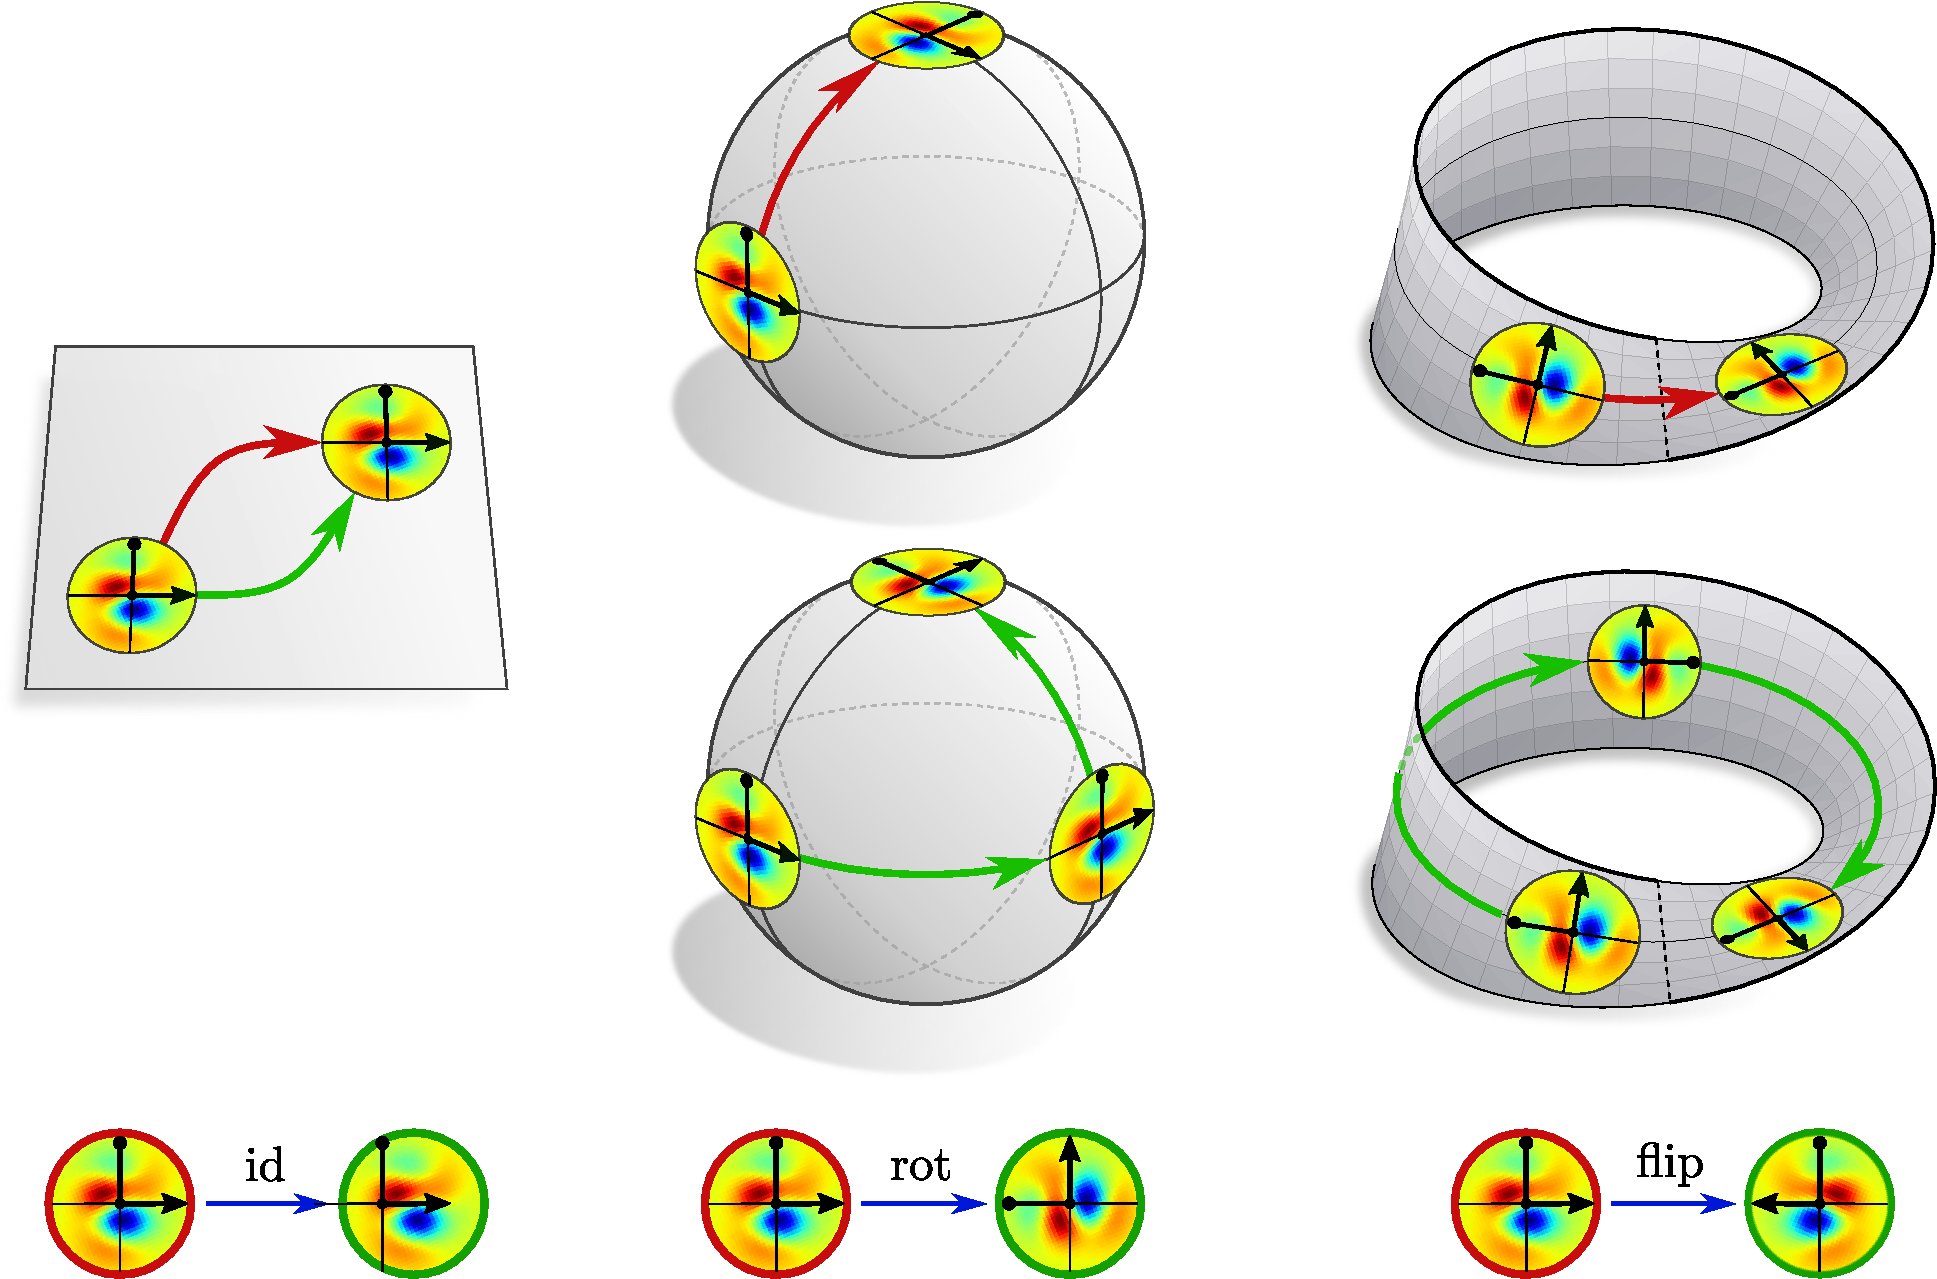
\includegraphics[width=.93\columnwidth]{figures/intro_transport_ambiguity.pdf}
    \caption{\small
        An intuition on the inherent ambiguity of weight sharing on manifolds.
        \ \ \emph{Left:}
        A common interpretation of weight sharing on the plane is to shift a kernel over the whole space.
        Since parallel transport is path independent on flat spaces, this is unambiguous.
        \ \ \emph{Middle:}
        On curved spaces, like the sphere, parallel transport is path dependent.
        Different paths result in kernels that are rotated relative to each other.
        \ \ \emph{Right:}
        The M\"obius strip is a non-orientable manifold.
        Different paths can therefore result in kernels that are reflected relative to each other.
        \ \ \emph{Bottom:}
        We formalize different kernel alignments by different choices of local reference frames of the corresponding tangent spaces.
        It is well known that no choice of reference frames (gauge) is preferred on general manifolds.
        Different coordinatizations are related by gauge transformations, which take values in the structure group $G$ of the manifold (the trivial group $G=\{e\}$ for the plane, rotation group $G=\SO2$ for the sphere and reflection group $G = \Flip$ for the M\"obius strip).
        Coordinate independent CNNs address the ambiguity of reference frames by applying $G$-steerable (gauge equivariant) convolution kernels.
    }
    \label{fig:weight_sharing_ambiguity}
\end{figure}


\section{Overview and visual intuition}
\label{sec:visual_intro}


The algebraic formulation of coordinate independent CNNs requires some familiarity with group theory, representation theory and differential geometry which might pose an obstacle for a non-technical audience.
However, most of our constructions and results are geometrically very intuitive and can be explained with a few visual examples.
This section attempts to give an overview and visual intuition about coordinate independent CNNs.

The following Section~\ref{sec:intro_overview_GM_conv} introduces $\GM$-coordinate independent convolutions on Riemannian manifolds.
Their equivariance under the action of isometries is discussed in Section~\ref{sec:intro_overview_isometry}.
Section~\ref{sec:intro_overview_G_structure_choice} comments on the factors that influence the choice of $G$-structure in the design of coordinate independent CNNs.




\toclesslab\subsection{\textit{G}-structures and \textit{GM}-coordinate independent convolutions}{sec:intro_overview_GM_conv}
Since convolutions are essentially characterized by their weight sharing property, a central question in this work is:
\vspace*{-1ex}
\begin{center}\it
    How should convolution kernels be shared over Riemannian manifolds?
    \footnote{
        This question applies more generally to any local template function, for instance biases or pointwise nonlinearities.
    }
\end{center}

%%%%%%%%%%%%%%%%%%%%%%%%%%%%%%%%%%%%%%%%%%%%%%%%%%%%%%%%%%%%%%%%%%%%%%%
%%%%%%%%%%%%%%%%%%%%%%%%%%%%%%%%%%%%%%%%%%%%%%%%%%%%%%%%%%%%%%%%%%%%%%%
\marginnote{} % somehow forces stuff on first page...
%%%%%%%%%%%%%%%%%%%%%%%%%%%%%%%%%%%%%%%%%%%%%%%%%%%%%%%%%%%%%%%%%%%%%%%
%%%%%%%%%%%%%%%%%%%%%%%%%%%%%%%%%%%%%%%%%%%%%%%%%%%%%%%%%%%%%%%%%%%%%%%


A common approach \marginnote{weight sharing via symmetries} is to share weights via the action of a symmetry group of the underlying space~\cite{Cohen2016-GCNN,Kondor2018-GENERAL}.
For instance, conventional CNNs share weights by translating kernels over the plane, while spherical CNNs share weights by rotating kernels over the sphere.
In order to share a kernel over the whole space, the action of the symmetry group needs to be \emph{transitive}.
As this is in general not the case for the isometries of Riemannian manifolds, this strategy is ruled out for our purpose.


The weight sharing on Euclidean spaces is often thought of as ``shifting'' a kernel over the space.
\marginnote{weight sharing via transport}
Since on flat spaces parallel transport is independent from the chosen path, this leads to an unambiguous alignment of kernels; see Fig.~\ref{fig:weight_sharing_ambiguity}~(left).
However, on curved or non-orientable spaces parallel transport becomes \emph{path dependent} and thus unsuitable for sharing weights.
Fig.~\ref{fig:weight_sharing_ambiguity} (middle and right) exemplifies this issue for the sphere and the M\"obius strip, where different paths lead to a different kernel alignment.


As the concept of ``kernel alignments'' is somewhat vague
\marginnote{weight sharing along frames}
we first need to make it mathematically precise:

\begin{minipage}{\textwidth}
\begin{center}\it
    We formalize the choice of kernel alignment at a point $p\in M$ \\
    as a choice of local reference frame (gauge)
    of the corresponding tangent space $\TpM$.
\end{center}
\end{minipage}

A reference frame at $p\in M$ is an ordered tuple $[e_1,\, \dots,\, e_d]$ of $d := \dim(M)$ linearly independent tangent vectors $e_i \in \TpM$, denoted as frame axes.
Since different frames at~$p$ are related by linear transformations, different choices of frames correspond to linear kernel deformations.
Fig.~\ref{fig:intro_kernel_alignment_trivial} shows two different choices of frame fields on~$M = \R^2$.
Sharing some convolution kernel along these frame fields results in the corresponding (convolutional) \emph{kernel fields}.


The identification of kernel alignments with reference frames raises the question:
\begin{center}\it
    To which extent is the choice of local reference frames on a (Riemannian) manifold ambiguous?
\end{center}
As elaborated in the following, the ambiguity of reference frames is determined by a $G$-structure with which the manifold is endowed.


\begin{SCfigure}
    \centering
    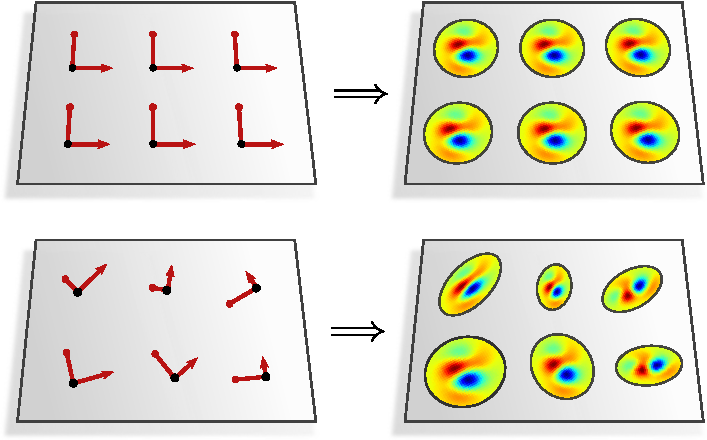
\includegraphics[width=.62\textwidth]{figures/intro_kernel_alignment_trivial.pdf}
    \captionsetup{width=.9\textwidth}
    \caption{\small
        A key property of convolutions is that they \emph{share weights} over the manifold.
        We identify the alignment of a kernel at $p\in M$ with a \emph{choice of reference frame} -- or \emph{gauge} -- of the corresponding tangent space~$\TpM$.
        Different \emph{frame fields} imply therefore different (convolutional) \emph{kernel fields}.
        \\[1ex]
        The choice of frames is often not unique.
        The ambiguity in this choice is formalized by $G$-\emph{structures}; see Fig.~\ref{fig:G_structures_intro}.
        To account for the arbitrariness of frames, the kernels are then required to be $G$-steerable (equivariant) as visualized in Figs.~\ref{fig:intro_steerable_kernel} and~\ref{fig:intro_kernel_alignment_reflect}.
        \\[0pt]
        }
    \label{fig:intro_kernel_alignment_trivial}
\end{SCfigure}





\subsubsection{\textit{G}-structures}
\label{sec:visual_intro_GM_subsub}

The space of \emph{all} possible frames of $\TpM$ is denoted as~$\FpM$.
\marginnote{frame bundle $\FM$}
Taken together, the frames of all tangent spaces form the \emph{frame bundle}~$\FM$; see Fig.~\ref{fig:frame_bundle}.
No specific choice of frames in $\FM$ is on a ``naked'' smooth manifold (without further geometric structure) preferred over each other, leaving the alignment of kernels maximally ambiguous.
In order to disambiguate frames and kernel alignments, the manifold needs to be equipped with \emph{additional geometric structure}.


A Riemannian manifold is equipped with a \emph{metric structure}.
\marginnote{metric structure $\OM$}
Providing an inner product (Riemannian metric) on the tangent spaces, this structure allows to single out those specific frames whose axes are \emph{orthonormal} to each other.
\emph{Gauge transformations}, i.e. transformations between choices of reference frames (see Figs.~\ref{fig:intro_gauge_isom_induction} (left) and~\ref{fig:gauge_trafos}), take then values in the \emph{orthogonal group}~$\O{d}$.
On Riemannian manifolds the alignment of kernels is therefore always disambiguated up to rotations and reflections.


Euclidean CNNs align convolution kernels (and thus frames)
\marginnote{$G$-structures $\GM$}
parallel to each other as visualized in Fig.~\ref{fig:intro_kernel_alignment_trivial} (top).
Spherical CNNs disambiguate kernel alignments usually up to rotations, that is, they assume a preferred handedness of reference frames.
The metric structure alone is insufficient to describe these settings, which suggests that these manifolds are equipped with \emph{further geometric structure besides the metric structure}.
We propose that the suitable mathematical framework is that of $G$-\emph{structures} and postulate:

\begin{minipage}{\textwidth}
\begin{center}\it
    The ambiguity in choosing reference frames (and thus kernel alignments) \\
    on a manifold $M$ is formalized by its $G$-structure $\GM$.
\end{center}
\end{minipage}

$G$-structures $\GM$ are \emph{bundles of distinguished reference frames} on $M$ such that the \emph{gauge transformations} between frames of the same tangent space take values in the \emph{structure group}~${G\leq\GL{d}}$.
Intuitively, one may think about the set $\GpM$ of frames of $\TpM$ as ``looking like'' $G$, however, without a distinguished origin.%
\footnote{
    $\GpM$ is a \emph{principal homogeneous space} of~$G$ (or $G$-torsor).
}


The frame bundle $\FM$ is itself a $G$-structure with~${G=\GL{d}}$, while the bundle of orthonormal frames $\OM$ is a $G$-structure (metric structure) with~${G=\O{d}}$.
Conventional Euclidean CNNs rely on the canonical frame field on $\R^d$ shown in Fig.~\ref{fig:G_structure_intro_a}, which is a $G$-structure for the trivial group~${G=\{e\}}$.
Fig.~\ref{fig:G_structures_intro} visualizes $G$-structures for further manifolds and structure groups.
An overview of common structure groups is found in Table~\ref{tab:G_structures} in Section~\ref{sec:local_G-structure_G-atlas}.


We will in the following always assume the Riemannian manifolds to be equipped with an additional $G$-structure next to its metric structure.%
\footnote{
    The $G$-structure needs to be compatible with the metric structure in that the distinguished frames in $\GM$ are a subset of the orthonormal frames in $\OM$ when $G<\O{d}$.
    Specifically for $G=\O{d}$, the $G$-structure $\GM$ coincides with the metric structure $\OM$ and adds no additional geometric information.
}
The particular choice of $G$-structure determines the properties of the neural network; we will comment on this choice in Section~\ref{sec:intro_overview_G_structure_choice} below.





%%%%%%%%%%%%%%%%%%%%%%%%%%%%%%%%%%%%%%%%%%%%%%%%%%%%%%%%%%%%%%%%%%%%%%%%%%%%%%%%%%%%%%%%%%%%%%%%%%%%%%%%%%
\afterpage{ % execute argument of this command *after* end of current page
\clearpage % clear any pending floats
%%%%%%%%%%%%%%%%%%%%%%%%%%%%%%%%%%%%%%%%%%%%%%%%%%%%%%%%%%%%%%%%%%%%%%%%%%%%%%%%%%%%%%%%%%%%%%%%%%%%%%%%%%
\begin{figure}
    \centering
    \vspace*{-4.ex}
    \begin{subfigure}[b]{0.26\textwidth}
	\centering
	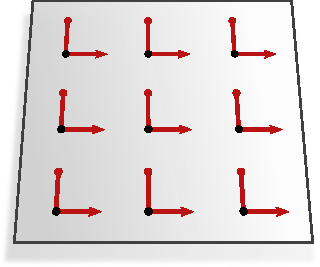
\includegraphics[width=1.\textwidth]{figures/G_structure_R2_1_big.pdf}
	\captionsetup{format=hang}
	\caption{\small
		\,$M = \R^2$,
		\,$G = \{e\}$
	}
	\label{fig:G_structure_intro_a}
\end{subfigure}
\hfill
\begin{subfigure}[b]{0.26\textwidth}
	\centering
	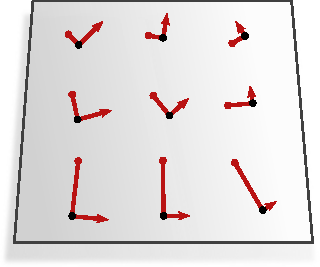
\includegraphics[width=1.\textwidth]{figures/G_structure_R2_5_big.pdf}
	\captionsetup{format=hang}
	\caption{\small
		\,$M = \R^2$,
		\,$G = \{e\}$
	}
	\label{fig:G_structure_intro_b}
\end{subfigure}
\hfill
\begin{subfigure}[b]{0.26\textwidth}
	\centering
	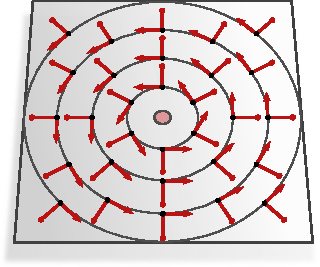
\includegraphics[width=1.\textwidth]{figures/G_structure_R2_no_origin_SO2_intro.pdf}
	\captionsetup{format=hang}
	\caption{\small
		\,$M = \R^2\backslash\{0\}$,
		\,$G = \{e\}$
	}
	\label{fig:G_structure_intro_c}
\end{subfigure}
\\[2ex]
%
%
%
%
\begin{subfigure}[b]{0.26\textwidth}
	\centering
	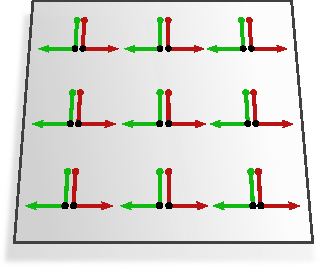
\includegraphics[width=1.\textwidth]{figures/G_structure_R2_3_big.pdf}
	\captionsetup{format=hang}
	\caption{\small
		\,$M = \R^2$,
		\,$G = \Flip$
	}
	\label{fig:G_structure_intro_d}
\end{subfigure}
\hfill
\begin{subfigure}[b]{0.26\textwidth}
	\centering
	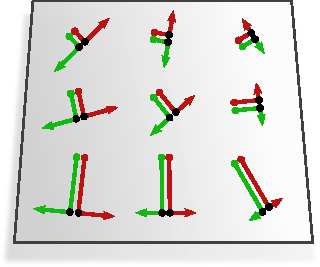
\includegraphics[width=1.\textwidth]{figures/G_structure_R2_6_big.pdf}
	\captionsetup{format=hang}
	\caption{\small
		\,$M = \R^2$,
		\,$G = \Flip$
	}
	\label{fig:G_structure_intro_e}
\end{subfigure}
\hfill
\begin{subfigure}[b]{0.26\textwidth}
	\centering
	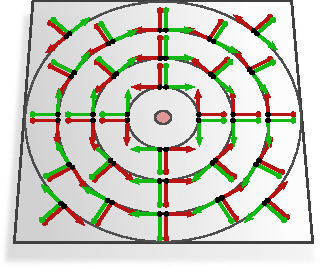
\includegraphics[width=1.\textwidth]{figures/G_structure_R2_no_origin_O2_intro.pdf}
	\captionsetup{format=hang}
	\caption{\small
		\,$M = \R^2\backslash\{0\}$,
		\,$G = \Flip$
	}
	\label{fig:G_structure_intro_f}
\end{subfigure}
\\[2ex]
%
%
%
%
\begin{subfigure}[b]{0.26\textwidth}
	\centering
	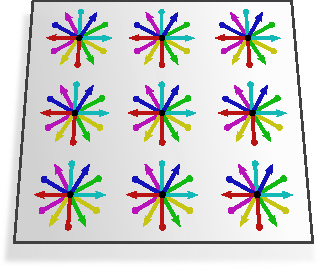
\includegraphics[width=1.\textwidth]{figures/G_structure_R2_2_big.pdf}
	\captionsetup{format=hang}
	\caption{\small
		\,$M = \R^2$,
		\,$G = \SO2$
	}
	\label{fig:G_structure_intro_g}
\end{subfigure}
\hfill
\begin{subfigure}[b]{0.26\textwidth}
	\centering
	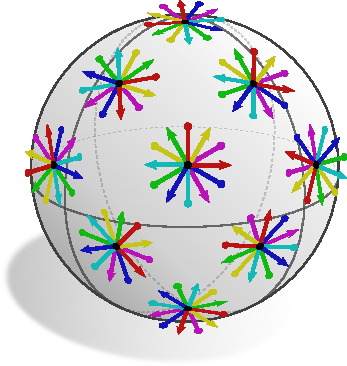
\includegraphics[width=.95\textwidth]{figures/G_structure_S2_1.pdf}
	\vspace*{-2ex}
	\captionsetup{format=hang}
	\caption{\small
		\,$M = S^2$,
		\,$G = \SO2$
	}
	\label{fig:G_structure_intro_h}
\end{subfigure}
\hfill
\begin{subfigure}[b]{0.26\textwidth}
	\centering
	\makebox[\textwidth][c]{ % center over-wide figure
		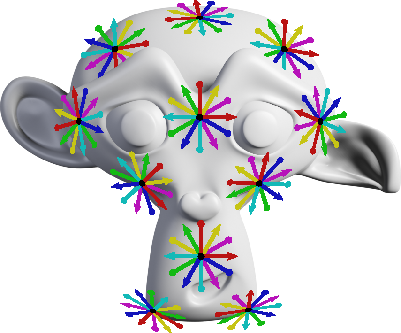
\includegraphics[width=1.12\textwidth]{figures/suzanne_SO2_structure.pdf}
	}
	\vspace*{-3.ex}
	\captionsetup{format=hang, width=1.1\textwidth}
	\caption{\small
		$M = \textup{``\href{https://en.wikipedia.org/wiki/Blender_(software)\#Suzanne}{\lr{Suzanne}}''}$\!,
		\ $G = \SO2$
	}
	\label{fig:G_structure_intro_i}
\end{subfigure}
\\[2ex]
%
%
%
%
\begin{subfigure}[b]{0.26\textwidth}
	\centering
	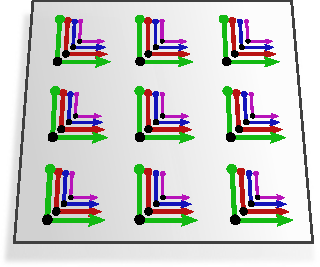
\includegraphics[width=1.\textwidth]{figures/G_structure_R2_4_big.pdf}
	\captionsetup{format=hang}
	\caption{\small
		\,$M = \R^2$,
		\,$G = \Scale$
	}
	\label{fig:G_structure_intro_j}
\end{subfigure}
\hfill
\begin{subfigure}[b]{0.26\textwidth}
	\centering
	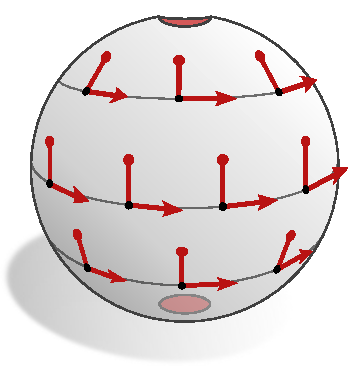
\includegraphics[width=.95\textwidth]{figures/G_structure_S2_2.pdf}
	\vspace*{-2ex}
	\captionsetup{format=hang}
	\caption{\small
		\,$M = S^2\backslash\text{\lr{poles}}$,
		\,$G = \{e\}$
	}
	\label{fig:G_structure_intro_k}
\end{subfigure}
\hfill
\begin{subfigure}[b]{0.26\textwidth}
	\centering
	\makebox[\textwidth][c]{ % center over-wide figure
		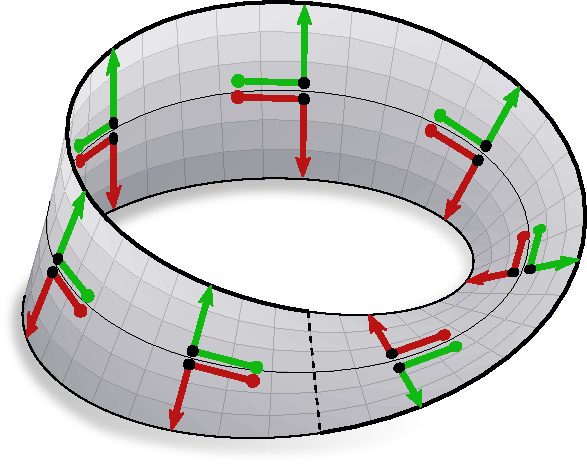
\includegraphics[width=1.1\textwidth]{figures/Mobius_R_structure.pdf}
	}
	\vspace*{-3.ex}
	\captionsetup{format=hang}
	\caption{\small
		\,$M = \textup{\lr{M\"obius}}$,
		\,$G = \Flip$
	}
	\label{fig:G_structure_intro_l}
\end{subfigure}
    \vspace*{1.5ex}
    \captionsetup{width=1.1\textwidth}
    \caption{\small
        Exemplary $G$-structures $\GM$ for different structure groups $G$ and on different manifolds $M$.
        The structure group $G$ signals which values gauge transformations can take, and therefore how ``big'' the subset of distinguished frames at each point~$p$ is.
        Fig.~\ref{fig:G_structure_intro_a} shows the canonical $\{e\}$-structure (frame field) of~$\R^2$, which corresponds to conventional Euclidean CNNs.
        The \mbox{$G$-structures} in
        Figs.~\ref{fig:G_structure_intro_d}, \ref{fig:G_structure_intro_g} and~\ref{fig:G_structure_intro_j}
        are constructed by adding reflected ($G=\Flip$), rotated ($G=\SO2$) and scaled ($G=\Scale$) frames, respectively.
        The corresponding $\GM$-convolutions are not only translation equivariant but equivariant under the action of affine groups~$\Aff(G)$.
        \mbox{$G$-structures} are usually not unique.
        Figs.~\ref{fig:G_structure_intro_b} and~\ref{fig:G_structure_intro_e} show alternative $G$-structures on~$\R^2$ (corresponding to an alternative metric relative to which their frames are orthonormal).
        They might not be practically relevant but demonstrate the flexibility of our framework.
        The $\{e\}$-structure in Fig.~\ref{fig:G_structure_intro_c} corresponds to polar coordinates.
        As $G$-structures are required to be continuous, we removed the origin~$0$ where polar coordinates are singular.
        One can once again define an $\Flip$-structure by adding reflected frames as shown in Fig.~\ref{fig:G_structure_intro_f}.
        These $G$-structures model convolutions on $\R^2\backslash\{0\}$ which are $\SO2$ and $\O2$-equivariant but not translation equivariant.
        Fig.~\ref{fig:G_structure_intro_h} shows the usual $\SO2$-structure on the embedded 2-sphere~$S^2$, which is underlying $\SO3$-equivariant spherical CNNs.
        Another popular choice is the $\{e\}$-structure in Fig.~\ref{fig:G_structure_intro_k}, which is induced by spherical coordinates.
        Note that this $\{e\}$-structure would be singular at the poles, which are therefore cut out.
        Continuous (i.e. non-singular) reductions of the structure group beyond~$\SO2$ are on the sphere topologically obstructed.
        $G$-steerable kernels with $G\geq\SO2$ are therefore strictly necessary for continuous convolutions on topological spheres like the mesh in Fig.~\ref{fig:G_structure_intro_i}.
        Fig.~\ref{fig:G_structure_intro_l} shows an $\Flip$-structure on the M\"obius strip.
        As the M\"obius strip is non-orientable, it does not admit a continuous reduction of the structure group beyond the reflection group~$G=\Flip$.
    }
    \label{fig:G_structures_intro}
\end{figure}
%%%%%%%%%%%%%%%%%%%%%%%%%%%%%%%%%%%%%%%%%%%%%%%%%%%%%%%%%%%%%%%%%%%%%%%%%%%%%%%%%%%%%%%%%%%%%%%%%%%%%%%%%%
\thispagestyle{empty}
\clearpage % force a page break
}
%%%%%%%%%%%%%%%%%%%%%%%%%%%%%%%%%%%%%%%%%%%%%%%%%%%%%%%%%%%%%%%%%%%%%%%%%%%%%%%%%%%%%%%%%%%%%%%%%%%%%%%%%%




\subsubsection{\textit{GM}-coordinate independent networks}
Our goal is
\marginnote{$\GM$-coordinate independence (covariance)}
to design neural networks on Riemannian manifolds with an additional $G$-structure.
If the structure group $G$ is non-trivial, \emph{no canonical choice of reference frames (gauge) exists} by definition.
However, in order to perform numerical computations, \emph{some} gauge, relative to which kernels and features are expressed, needs to be chosen.
Since this choice is inherently arbitrary we demand that the networks' inference should ultimately not depend on it, that is, we require:
\begin{center}\it
    Neural networks on a Riemannian manifold with $G$-structure $\GM$ \\
    should be based on ``$\GM$-coordinate independent'' operations.
\end{center}
``$\GM$-coordinate independence'' means hereby that \emph{all geometric quantities and functions between them should be equally well expressible in any gauge}, i.e. relative to any choice of reference frames of the $G$-structure.
The specific case of tangent vector coefficients and gauge transformations between them is visualized in Fig.~\ref{fig:gauge_trafos}.
Fig.~\ref{sec:gauges_TpM_functions} shows an example of a linear map and its coordinate independent representation in terms of matrices relative to different frames.


Note that the requirement for $\GM$-coordinate independence is quite flexible:
for $G=\GL{d}$ one has $\GM=\FM$ and therefore the maximal level of coordinate independence.
At the other end of the spectrum of structure groups one has $G=\{e\}$, for which $\GM$ is a fixed frame field and $\GM$-coordinate independence reduces to an explicit coordinate dependence.
The freedom of choosing arbitrary $G$-structures allows for a precise control over the networks' coordinate independence,
which varies in practice widely; see for instance Table~\ref{tab:network_instantiations} in Part~\ref{part:literature_review}.


Our networks process \emph{feature vector fields} on the manifold.
\marginnote{$G$-associated feature vector fields}
Feature vectors are \emph{coordinate free} geometric quantities like e.g. tangent vectors.
Relative to a chosen frame (gauge) they may be represented by \emph{numerical coefficient vectors}.
The demand for $\GM$-coordinate independence requires the numerical coefficients in different gauges to encode the same information content.
This is naturally achieved by associating the features with a group representation~$\rho$ of the structure group~$G$ which determines their coefficients' transformation behavior under gauge transformations:
\begin{center}\it
    Feature vector fields are associated with a $G$-representation $\rho$ which specifies \\
    the transformation law of their numerical coefficients when transforming between reference frames.
    \\[1ex]
    Technically speaking, feature fields are sections of $G$-associated feature vector bundles.
\end{center}
Typical examples are scalar fields, tangent vector fields or other tensor fields, however, any transformation law is admissible and can be chosen by the user.
Other common choices for~$\rho$ in the deep learning context are irreducible or regular representations;
more examples are listed in Table~\ref{tab:network_instantiations} in Part~\ref{part:literature_review}.


We want to emphasize that the requirement for $\GM$-coordinate independence is a mere \emph{consistency condition}, guaranteeing that different observers (frames) agree on the same coordinate free geometric observation.
It~does \emph{not} constrain the set of admissible functions in any way, but only how their expressions relative to different frames relate.
In particular, \emph{$\GM$-coordinate independent neural networks are in general not required to be gauge equivariant}.
A requirement for gauge equivariance follows when simultaneously demanding weight sharing and coordinate independence, that is, $\GM$-coordinate independent convolutions rely on gauge equivariant kernels.



\begin{SCfigure}[2.5]
    \centering
    \small
    $\begin{array}{c@{\hspace{2pt}}c}
        \rotatebox{-90}{
            \includegraphicstotab[width=.12\textwidth]{figures/kernels/K_symmetric.png}
        } &
        \reflectbox{\rotatebox{-90}{
            \includegraphicstotab[width=.12\textwidth]{figures/kernels/K_antisymmetric.png}
        }} \\[60pt]
        \textup{scalar} & \textup{scalar} \\
        \updownarrow & \updownarrow \\
        \textup{scalar} & \textup{pseudoscalar}
        \\[-2pt] ~
    \end{array}$
    \hspace*{-2.5ex}
    \caption[]{\small
        Exemplary $G$-steerable kernels for the group $G=\Flip$ of reflections along the first frame axis (parity transformations).
        The kernels' equivariance constraints depend on the field types $\rhoin$ and $\rhoout$ of the convolution input and output.
        Scalar and pseudoscalar fields are described by the trivial representation and the sign-flip representation of $\Flip$, respectively.
        Steerable kernels which map between such fields are constrained to be symmetric or antisymmetric.
        \\[1ex]
        Note that steerable kernels are in general not scalar-valued but ${\cout \!\times\! \cin}$-matrix valued, where $\cout$ and $\cin$ are the dimensionalities of the output and input feature vectors, respectively.
        A derivation and more examples for other (higher-dimensional) field types of $G=\Flip$ are found in Section~\ref{sec:mobius_kernel_spaces} and Table~\ref{tab:reflection_steerable_kernels}.
        Steerable kernels for $G=\SO2$ or $G=\SO3$ are constructed from circular \cite{Weiler2019_E2CNN,Worrall2017-HNET,Weiler2018SFCNN} or spherical \cite{3d_steerableCNNs,Thomas2018-TFN} harmonics.
        If~$G$ is compact, $G$-steerable kernels are described by a generalization of the Wigner-Eckart theorem~\cite{lang2020WignerEckart}.
        \\[-20pt]
    }
    \label{fig:intro_steerable_kernel}
\end{SCfigure}





\subsubsection{\textit{GM}-coordinate independent convolutions}
We come back to our initial question
\marginnote{$\GM$-coordinate independent weight sharing $~\mkern22mu~\Longleftrightarrow$ $G$-steerability}
about how to share a convolution kernel given that its alignment is inherently ambiguous when the structure group~$G$ is non-trivial.
As the convolution operation should be $\GM$-coordinate independent, the underlying weight sharing procedure needs to be independent from arbitrary choices of reference frames as well.
Aligning the kernel along different frames of the $G$-structure at some point~$p$ should therefore always yield equivalent results.
We demonstrate that the $\GM$-coordinate independence of the weight sharing process imposes a \emph{gauge equivariance constraint} (``$G$-steerability'') on the convolution kernels:
\begin{align*}
    \qquad
    \begin{array}{r@{}}
        \GM \mkern.0mu \rule[2.25pt]{4pt}{.5pt} \mkern1.5mu \textit{coordinate independence}\ \ \\[4pt]
        \textit{weight sharing}\ \ 
    \end{array}
    \Bigg\}
    \mkern-10mu \boldsymbol{\longrightarrow}
    \ G \mkern.75mu \rule[2.25pt]{4pt}{.5pt} \mkern1.5mu \textit{steerability}\ \ \textit{(gauge equivariance)}
\end{align*}
Fig.~\ref{fig:intro_steerable_kernel} and Table~\ref{tab:reflection_steerable_kernels} show examples of reflection steerable kernels.
The equivariance (steerability) constraint enforces some type of $G$-symmetry which ensures that the \emph{kernel responses transform predictably} under gauge transformations.
An intuitive demonstration of how $G$-steerable kernels resolve the ambiguity of reference frames is given in Fig.~\ref{fig:intro_kernel_alignment_reflect}.


%%%%%%%%%%%%%%%%%%%%%%%%%%%%%%%%%%%%%%%%%%%%%%%%%%%%%%%%%%%%%%%%%%%%%%%%%%%%%%%%%%%%%%%%%%%%%%%%%%%%%%%%%%%%%%%%%%%%%%%%%
\begin{samepage}
$\GM$-coordinate independent convolutions (or $\GM$-\emph{convolutions} in short)
{\setlength{\marginparwidth}{2.5cm}% prevent marginnote from moving to next line when being too wide
\marginnote{$\GM$-convolutions}}%
are defined as convolutions with $G$-steerable kernels:
\begin{center}\it
    A $\GM$-convolution with a $G$-steerable kernel $K$ processes features by applying this \\
    kernel at each point $p\in M$ relative to an arbitrary choice of reference frame in $\GpM$. \\
\end{center}
\end{samepage}
%%%%%%%%%%%%%%%%%%%%%%%%%%%%%%%%%%%%%%%%%%%%%%%%%%%%%%%%%%%%%%%%%%%%%%%%%%%%%%%%%%%%%%%%%%%%%%%%%%%%%%%%%%%%%%%%%%%%%%%%%
The arbitrariness of the chosen gauge is thereby ensured by the kernel's $G$-steerability.
While being constructed in local coordinates, 
$\GM$-convolutions correspond to well defined \emph{coordinate free} convolution operation on the manifold.


Not only convolution kernels but \emph{any shared template function is required to be gauge equivariant} in order to preserve $\GM$-coordinate independence.
Section~\ref{sec:pointwise_operations} derives the equivariance constraints on shared biases, \onexone\ kernels and nonlinearities.
Note that the equivariance constraints on shared template functions can be viewed as a form of weight sharing over $G$-related reference frames
-- the ambiguity of sharing weights over the manifold~$M$ is therefore resolved by extending weight sharing over the whole $G$-structure~$\GM$.



\begin{figure}
    \centering
    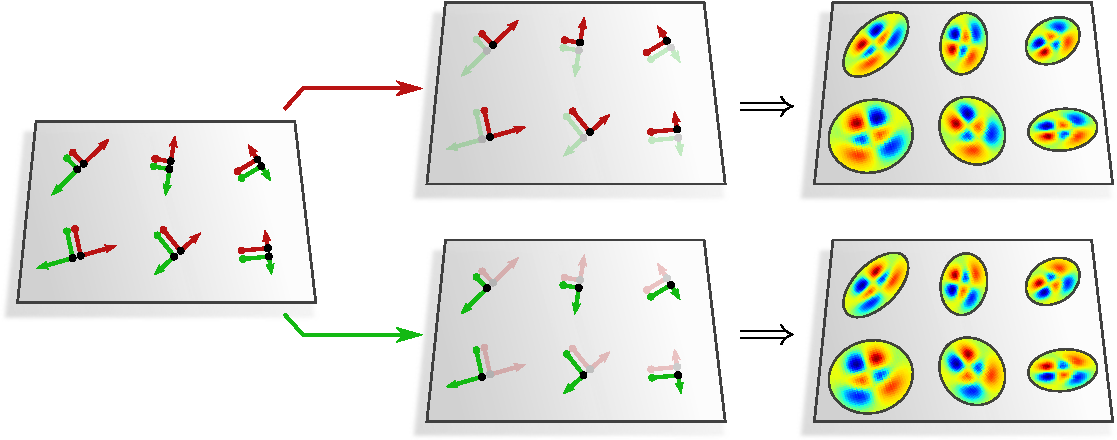
\includegraphics[width=1.\textwidth]{figures/intro_kernel_alignment_reflect.pdf}
    \caption{\small
        Sharing an $\Flip$-steerable kernel according to a given $\Flip$-structure $\RM$ over a manifold~$M = \R^2$.
        There are two continuous gauges (red and green) along which the kernel could be shared.
        Due to its $\Flip$-equivariance, the particular choice is ultimately irrelevant.
        The visualized kernel is antisymmetric and maps therefore between scalar and pseudoscalar fields.
        It is easily verified that this is indeed the case:
        the numerical coefficients of a scalar input field stay invariant under gauge transformations but the kernels are reflected.
        As they are antisymmetric, their responses will negate -- which is the transformation law of the numerical coefficients of a pseudoscalar field.
        A similar reasoning holds for mappings from pseudoscalars to scalars.
        How could we have mapped from scalars to scalars?
        In this case both the input and the output should be gauge invariant, requiring the kernel to be symmetric instead of antisymmetric.
        Symmetric kernels map furthermore between pseudoscalar fields.
    }
    \label{fig:intro_kernel_alignment_reflect}
\end{figure}





\toclesslab\subsection{Equivariance under global symmetries of the manifold}{sec:intro_overview_isometry}

\begin{SCfigure}
    \centering
    \hspace*{2ex}
    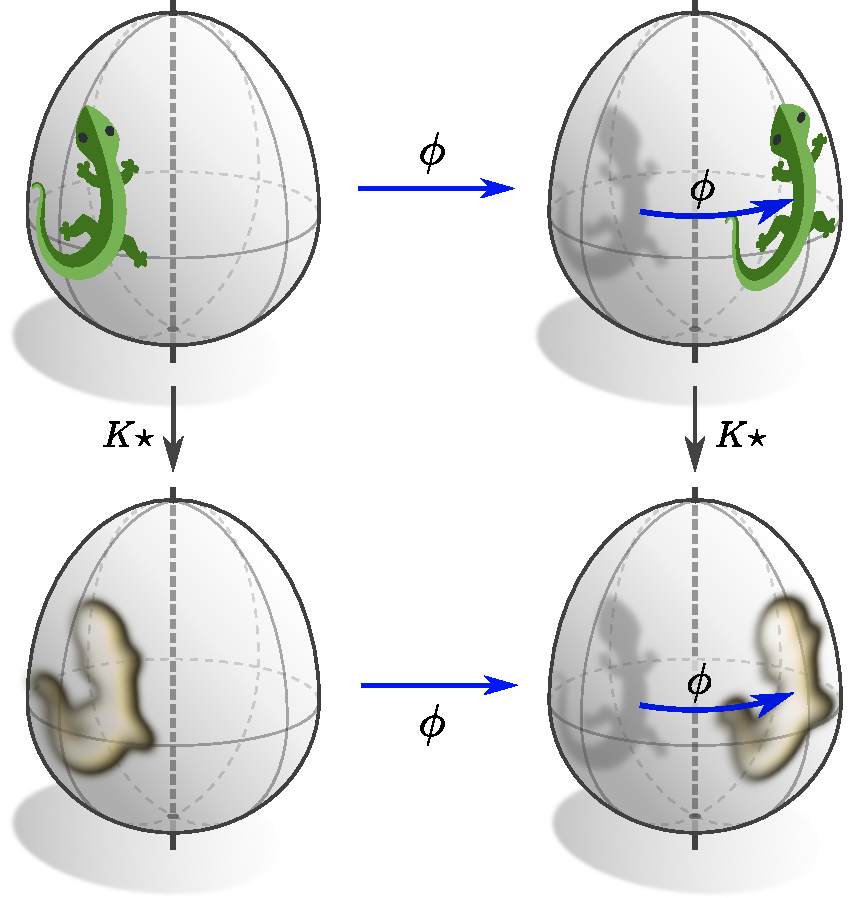
\includegraphics[width=.5\textwidth]{figures/lizard_conv_egg_intro.pdf}
    \captionsetup{width=.9\textwidth}
    \caption[]{\small
        Visualization of an isometry equivariant $\GM$-convolution.
        An isometry $\phi$ acts via pushforward on feature fields.
        The $\GM$-convolution $K\star$ with a $G$-steerable kernel $K$ is said to be equivariant w.r.t. this isometry when the convolution response of a transformed input ($\rightarrow,\downarrow$) agrees with the pushforward of the untransformed input's response ($\downarrow,\rightarrow$).
        \\[1ex]
        $\GM$-convolutions are equivariant w.r.t. the (sub)group $\IsomGM$ of isometries that are symmetries of the $G$-structure.
        The visualized azimuthal rotation equivariance requires therefore a $G$-structure that is invariant under rotations around the polar axis -- this condition is for instance met by the analogue of the spherical $G$-structures in Figs.~\ref{fig:G_structure_intro_h} and~\ref{fig:G_structure_intro_k} on the egg.
        The isometry group of the egg-shaped manifold contains not only rotations but also reflections.
        To achieve reflection equivariance, the $G$-structures would additionally have to contain reflected frames and the $\GM$-convolution would have to apply reflection steerable kernels.
        {\\
        \color{gray}
        \scriptsize
            (Lizards adapted under the Creative Commons Attribution 4.0 International
            \href{https://github.com/twitter/twemoji/blob/gh-pages/LICENSE-GRAPHICS}{\underline{license}}
            by courtesy of Twitter.)
        }
        \\[-16pt]
        }
    \label{fig:lizard_conv_egg_intro}
\end{SCfigure}


Convolution operations are often designed to be equivariant w.r.t. the symmetries of the underlying space \cite{Cohen2016-GCNN,Kondor2018-GENERAL}.
The symmetries of a Riemannian manifold form its \emph{isometry group} $\IsomM$, which is the group of all distance preserving maps~${\phi:M\to M}$.
Isometries act naturally on geometric quantities like feature vectors by ``moving them along'' with the isometry action (pushforward); see Fig.~\ref{fig:intro_gauge_isom_induction} (middle).
Despite only being designed to be equivariant under local gauge transformations,
$\GM$-convolutions are equivariant w.r.t. the action of specific isometry subgroups $\IsomGM \leq \IsomM$ on feature fields.
These subgroups $\IsomGM$ contain those \emph{isometries which are symmetries of the $G$-structure}.
The design of isometry equivariant $\GM$-convolutions is therefore linked to the design of invariant $G$-structures.
Fig.~\ref{fig:lizard_conv_egg_intro} visualizes the idea of an isometry equivariant $\GM$-convolution graphically.


We will in the following briefly discuss symmetry constraints which the requirement of isometry equivariance imposes on kernel fields, i.e. on the neural connectivity.
These conditions on the kernel fields correspond to symmetry constraints on the $G$-structures along which convolution kernels are shared.
We will finally comment on why $\GM$-convolutions are only isometry equivariant and are in general not equivariant w.r.t. more general diffeomorphisms.






\pagebreak






\subsubsection{Isometry invariant kernel fields}
\label{sec:visual_intro_inv_kernel_fields}

The equivariance properties of a neural network
\marginnote{kernel field transforms}
depend ultimately on symmetries in its neural connectivity~\cite{ravanbakhsh2017EquivarianceParameterSharing}.
For convolutional networks this amounts to \emph{symmetry constraints on the kernel field}.
To study these constraints in full generality, we do not require the kernel fields to be \emph{convolutional}, i.e. determined by a single shared kernel,
but assume \emph{general kernel fields} which may apply a different kernel at each point in space.
We denote the corresponding network layers as \emph{``kernel field transforms''}:%
\footnote{
    Kernel field transforms are in the computer vision literature sometimes called ``\emph{locally connected networks}''.
}
\begin{center}\it
    ``Kernel field transforms'' are similar to $\GM$-convolutions but may apply a different kernel at every point. \\
    They are therefore parameterized by general kernel fields.
\end{center}
$\GM$-convolutions are specific kernel field transforms with $\GM$-convolutional kernel fields.
The general results for isometry equivariant kernel field transforms translate therefore immediately to $\GM$-convolutions.


Theorem~\ref{thm:isometry_equivariant_kernel_field_trafos} proves
\marginnote{isometry invariant kernel~fields}
that the invariance of a kernel field under the isometry action and the equivariance of the corresponding kernel field transform imply each other:
\begin{center}\it
    isometry invariant kernel field
    $\quad \Longleftrightarrow \quad$
    isometry equivariant kernel field transform
\end{center}
Invariant kernel fields are constrained in two qualitatively different ways:
Firstly, kernels need to be shared over the \emph{isometry orbits}.
Secondly, the shared kernels are themselves constrained by the \emph{stabilizer subgroup} of the corresponding orbit.
Note that the full, symmetric kernel field can be recovered from a single representative kernel for each orbit --
Theorems~\ref{thm:tangent_quotient_repr_kernel_fields} and~\ref{thm:manifold_quotient_repr_kernel_fields} formalize this statement by proving isomorphisms between invariant kernel fields on the manifold and kernel fields on quotient spaces under the isometry action.

\begin{figure}
    \hspace{1.ex}
    \begin{subfigure}[b]{0.24\textwidth}
        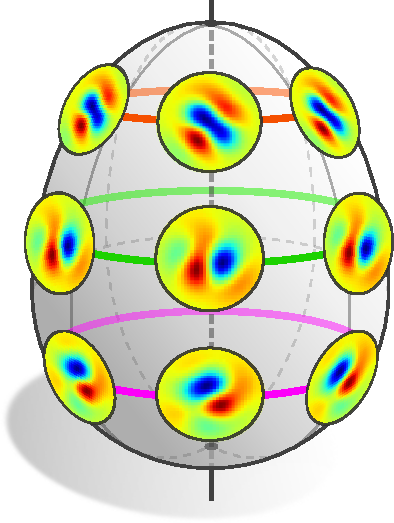
\includegraphics[width=.92\textwidth]{figures/isometry_egg_intro_symmetric.pdf}
        \vspace*{-.5ex}
        \captionsetup{format=hang, width=.7\textwidth}
        \caption{\small
            $\SO2$-invariant kernel field
        }
        \label{fig:isom_invariant_kernel_field_intro_SO2}
    \end{subfigure}
    \hspace*{1.5ex}
    \begin{subfigure}[b]{0.24\textwidth}
        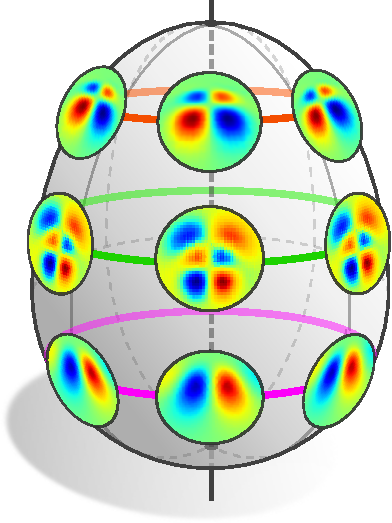
\includegraphics[width=.92\textwidth]{figures/isometry_egg_intro_antisymmetric.pdf}
        \vspace*{-.5ex}
        \captionsetup{format=hang, width=.7\textwidth}
        \caption{\small
            $\O2$-invariant kernel field
        }
        \label{fig:isom_invariant_kernel_field_intro_O2}
    \end{subfigure}
    \par
    \vspace*{\dimexpr-\parskip-158.pt\relax}% Skip backwards over last left-aligned image
    \parshape 17 % Set flow of caption: N lines...
        .55\textwidth .45\textwidth % First N-1 start @ .55\textwidth with a width of .45\textwidth
        .55\textwidth .45\textwidth
        .55\textwidth .45\textwidth
        .55\textwidth .45\textwidth
        .55\textwidth .45\textwidth
        .55\textwidth .45\textwidth
        .55\textwidth .45\textwidth
        .55\textwidth .45\textwidth
        .55\textwidth .45\textwidth
        .55\textwidth .45\textwidth
        .55\textwidth .45\textwidth
        .55\textwidth .45\textwidth
        .55\textwidth .45\textwidth
        .55\textwidth .45\textwidth
        .55\textwidth .45\textwidth
        .55\textwidth .45\textwidth
        .01\textwidth .98\textwidth % the last (N-th) line flows from 0 to .99 = .62+.37 = .01+.98 ad infinitum
    \makeatletter
    \setcounter{\@captype}{\value{\@captype}-1} % \setcounter{CounterName}{number}
    \refstepcounter{\@captype}% Increase float/caption counter
    \addcontentsline{\csname ext@\@captype\endcsname}{\@captype}% Add content to "List of..."
        {\protect\numberline{\csname the\@captype\endcsname}{ToC entry}}%
    \small % switch to small font for caption and Figure XX:
    \csname fnum@\@captype\endcsname: % Float caption + #
    \makeatother
    \hyphenpenalty = 300 % default should be 50, however, without setting this parameter no hyphens occurred
    % Actual caption
        \emph{Kernel field transforms} are similar to $\GM$-convolutions but may apply a different kernel at each point.
        Theorem~\ref{thm:isometry_equivariant_kernel_field_trafos} proves that \emph{isometry equivariant kernel field transforms} are in one-to-one correspondence with \emph{isometry invariant kernel fields}.
        This implies
        1) weight sharing over the \emph{isometry orbits} (colored rings) and
        2) a constraint on the kernels to be steerable w.r.t. the \emph{stabilizer subgroup} of their respective orbit.
        Fig.~\ref{fig:isom_invariant_kernel_field_intro_SO2} shows an $\SO2$-invariant kernel field on an egg-shaped manifold.
        Different orbits are free to use different kernels without compromising $\SO2$-equivariance.
        The kernels themselves are unconstrained since the stabilizer subgroups of the $\SO2$ action on the orbits are trivial (except for at the poles).
        Fig.~\ref{fig:isom_invariant_kernel_field_intro_O2} visualizes the case of an $\O2$-invariant kernel field.
        The orbits are the same, however, the stabilizer subgroups impose a reflectional equivariance constraint.
        Note that the notion of invariance depends on the group action on the kernel, Def.~\ref{dfn:isometry_action_kernel_fields}, which depends in turn on the chosen feature field representations.
        The antisymmetric kernels are in this sense invariant under reflections.
    \label{fig:isom_invariant_kernel_field_intro}
\end{figure}


Figs.~\ref{fig:isom_invariant_kernel_field_intro_SO2} and~\ref{fig:isom_invariant_kernel_field_intro_O2}
\marginnote{examples}
exemplify these results for an egg-shaped manifold, whose isometries are rotations and reflections around the vertical axis.
A general kernel field transform could apply any kernel field.
If only $\SO2$ isometry equivariance is required (no reflections), the orbits are rings around the egg and the stabilizer subgroup of the $\SO2$-action on these orbits is trivial; see Fig.~\ref{fig:isom_invariant_kernel_field_intro_SO2}.%
\footnote{
    We are for brevity ignoring the poles, where the stabilizer subgroup is $\SO2$ in Fig.~\ref{fig:isom_invariant_kernel_field_intro_SO2} and $\O2$ in Fig.~\ref{fig:isom_invariant_kernel_field_intro_O2}.
}
The isometry invariant kernel field is therefore sharing unconstrained kernels over these orbits.
Fig.~\ref{fig:isom_invariant_kernel_field_intro_O2} shows an $\O2$-invariant kernel field.
The orbits, and therefore the spatial weight sharing pattern, are here the same as in the previous case.
However, the stabilizer subgroup of the $\O2$-action on the orbits is the reflection group.
The kernels are therefore constrained to be reflection steerable, with the exact constraint depending on the types $\rhoin$ and $\rhoout$ of the input and output feature field.


An interesting special case
\marginnote{homogeneous spaces}
is that of manifolds which are \emph{homogeneous spaces} of their isometry group.
In this case there is only one single orbit, such that an invariant kernel field is determined by a \emph{single shared (convolution) kernel}.
Theorem~\ref{thm:GM_conv_homogeneous_equivalence} proves:
\begin{center}\it
    Isometry equivariant kernel field transforms on homogeneous spaces are necessarily convolutions.
\end{center}
The kernels are again required to be steerable w.r.t. the stabilizer subgroup of the isometry action.
This recovers the results of \citet{Kondor2018-GENERAL}, \citet{Cohen2019-generaltheory} and \citet{bekkers2020bspline}, who investigated group equivariant CNNs on homogeneous spaces; see Appendix~\ref{apx:homogeneous_conv} for an in-depth comparison.








\subsubsection{Isometry equivariance of \textit{GM}-convolutions}
\label{sec:visual_intro_isom_equiv_conv}

\paragraph{Isometry invariant \textit{G}-structures:}
$\GM$-convolutions are specific kernel field transforms
\marginnote{isometry invariant $G$-structures}
which rely on $\GM$-convolutional kernel fields.
They are therefore isometry equivariant if the $\GM$-convolutional kernel field is invariant under the isometry action.
Recall that $\GM$-convolutional kernel fields are defined by sharing some $G$-steerable kernel along (arbitrary) frames of the $G$-structure.
Their symmetries (isometries) coincide therefore with those of the $G$-structure.
\begin{center}\it
    We define $\IsomGM \leq \IsomM$ as the subgroup of those isometries which are \\
    symmetries of the $G$-structure $\GM$ (principal bundle automorphisms).
\end{center}
\begin{minipage}{\textwidth}
It follows that
\begin{center}\it
    $\GM$-convolutional kernel fields are $\IsomGM$-invariant.
\end{center}
\vspace*{1ex}\end{minipage}
\begin{minipage}{\textwidth}
As a consequence, which is proven rigorously in Theorem~\ref{thm:isom_equiv_GM_conv}, we find:
\begin{center}\it
    $\GM$-convolutions are $\IsomGM$-equivariant.
\end{center}
\vspace*{1ex}\end{minipage}
The design of isometry equivariant $\GM$-convolutions is therefore reduced to the design of isometry invariant $G$-structures.
Fig.~\ref{fig:intro_invariant_kernel_fields_plane} shows two examples of $G$-structures $\GM$ and corresponding $\GM$-convolutional kernel fields, which share the same symmetries.
For more examples we refer back to the $G$-structures in Fig.~\ref{fig:G_structures_intro}.
Note that $\IsomGM$ contains for $G=\O{d}$ (or supergroups of it) all possible isometries, implying that the corresponding $\GM$-convolutions are fully $\IsomM$-equivariant.
A similar statement holds for $G=\SO{d}$ and orientation preserving isometries.

\begin{SCfigure}
    \centering
    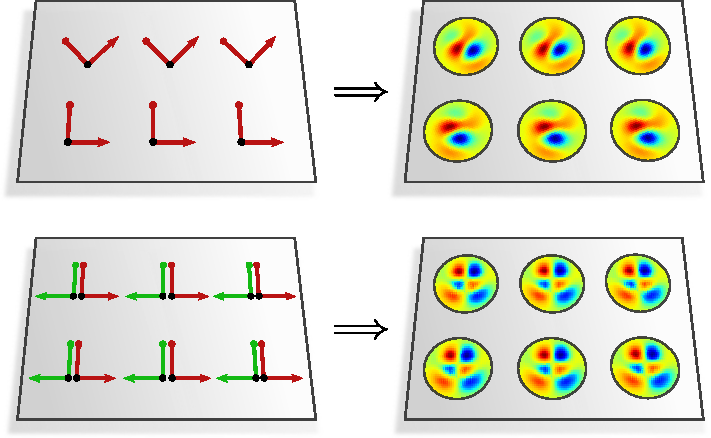
\includegraphics[width=.62\textwidth]{figures/intro_invariant_kernel_fields_plane.pdf}
    \captionsetup{width=.92\textwidth}
    \caption{\small
        \mbox{$\GM$-convolutional} kernel fields are constructed by sharing some $G$-steerable kernel along (arbitrary) frames of the \mbox{$G$-structure} $\GM$.
        The symmetries of the kernel fields agree therefore with those of the $G$-structure, i.e. with $\IsomGM$.
        The $\{e\}$-structure that is visualized at the top corresponds thus to a \mbox{$\GM$-convolution} which is equivariant w.r.t. translations in horizontal direction but not in vertical direction.
        As the \mbox{$\Flip$-structure} that is visualized at the bottom is invariant under arbitrary translations and horizontal reflections, the implied \mbox{$\GM$-convolution} is translation and reflection equivariant.
        \\[-5pt]
        }
    \label{fig:intro_invariant_kernel_fields_plane}
\end{SCfigure}






\paragraph{Isometry induced gauge transformations:}

The argumentation in terms of invariant kernel fields
\marginnote{isometry induced gauge transformations}
and invariant $G$-structures did not rely on any choice of gauge but was formulated in a purely geometric, \emph{coordinate free} setting.
An alternative viewpoint explains the isometry equivariance of $\GM$-convolutions in coordinates, where isometries act via induced gauge transformations.
These gauge transformations are explained away by the kernel's $G$-steerability, which provides a link between the concepts of \emph{gauge equivariance} and \emph{isometry equivariance}.
We elaborate in the following concisely on this alternative viewpoint.


When being expressed \emph{relative to local reference frames}, isometries can be thought of as acting via \emph{induced gauge transformations} on feature vector coefficients.
Fig.~\ref{fig:intro_gauge_isom_induction} (right) visualizes this concept:
assume that we picked reference frames at some point $p$ and at its image $\phi(p)$ under the action of an isometry~$\phi$.
The isometry pushes a feature from $p$ to $\phi(p)$.
As the Riemannian geometries around $p$ and $\phi(p)$ are indistinguishable, the only thing that changed from the viewpoint of the feature vector is with respect to which reference frame it is being expressed.
This change of frames is the isometry induced gauge transformation.

\begin{figure}
    \centering
    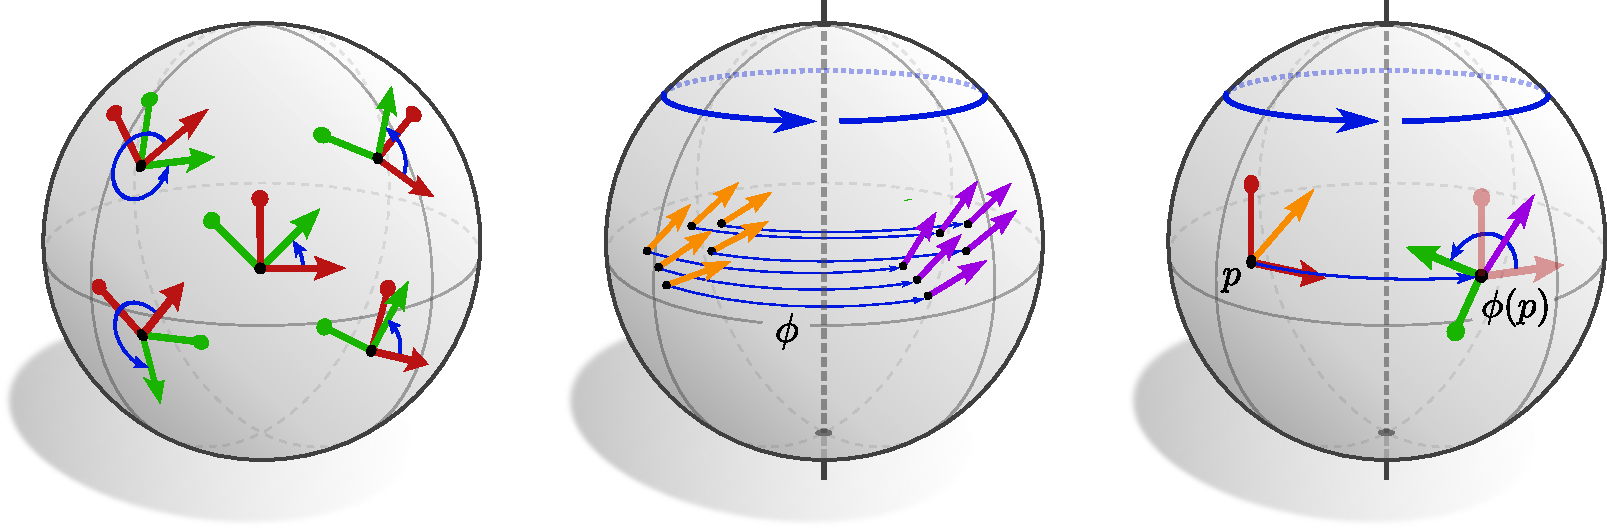
\includegraphics[width=.98\columnwidth]{figures/intro_gauge_isom_equiv.pdf}
    \vspace*{-1ex}
    \caption{\small
        Gauge transformations, isometries and their mutual relation.
        \ \ \emph{Left:}
        A gauge is a choice of local reference frames (a frame field), relative to which geometric quantities may be expressed.
        If the manifold's structure group $G$ is non-trivial, the choice of gauge is not unique but many equivalent choices exist.
        Different choices of gauges (red or green) are related by gauge transformations (blue) which are by definition taking values in the structure group~$G$.
        Visualized are orthonormal, right-handed frames, for which the gauge transformations are $G=\SO{2}$-valued.
        \ \ \emph{Middle:}
        Isometries are the symmetries of Riemannian manifolds.
        They are defined as distance preserving functions $\phi: M \to M$, mapping the manifold to itself.
        Isometries act via pushforward on tangent vectors, reference frames and feature vectors.
        While gauge transformations are passive coordinate transformations, isometries are actively moving points and geometric quantities over the manifold.
        \ \ \emph{Right:}
        When being expressed relative to local reference frames, the action of isometries can be thought of as inducing gauge transformations.
        Assume frames at $p$ (red) and $\phi(p)$ (green) to be given.
        A geometric quantity at $p$ (orange) is by the isometry pushed to $\phi(p)$ (purple).
        Since $\phi$ is an isometry, the Riemannian geometry around $p$ and $\phi(p)$ is indistinguishable, however, the pushforward of the geometric quantity is expressed relative to a new reference frame (green instead of red).
        One can therefore view isometries as inducing gauge transformations.
        If these induced gauge transformations take values in the structure group $G$, they are explained away by the $G$-steerability (gauge equivariance) of convolution kernels -- $\GM$-convolutions are then isometry equivariant.
        This condition is always met for $G\geq\O{d}$.
    }
    \label{fig:intro_gauge_isom_induction}
\end{figure}


Recall that $\GM$-convolutions apply the same $G$-steerable kernel at each point of the manifold.
The kernel's $G$-equivariance accounts for any $G$-valued (induced) gauge transformation, such that:
\begin{center}\it
    If an isometry induces gauge transformations that take values in the structure group~$G$, \\
    then any $\GM$-convolution is equivariant w.r.t. this isometry.
\end{center}


The induced gauge transformations for general isometries might not take values in the chosen structure group~$G$.
For instance, the $G$-structures in Figs.~\ref{fig:G_structure_intro_a} and~\ref{fig:G_structure_intro_d} have structure groups $G=\{e\}$ and $G=\Flip$, respectively, but rotations of $M=\R^2$ induce $\SO2$- or $\O2$-valued gauge transformations.
However, if an isometry is a symmetry of the $G$-structure, i.e. an element of $\IsomGM$, it maps frames in~$\GM$ to frames in~$\GM$.
Since frames in~$\GM$ are related by $G$-valued gauge transformations it follows that:
\begin{center}\it
    Isometries in $\IsomGM$ induce gauge transformations that take values in the structure group $G$.
\end{center}
This implies that $\GM$-convolutions are $\IsomGM$-equivariant, as already found in the coordinate free setting.
While this alternative viewpoint is less geometrically intuitive, it emphasizes the role of the kernels' $G$-steerability in the networks' isometry equivariance.




\subsubsection{Diffeomorphisms, isometries and affine transformations:}
\label{sec:visual_intro_diffeo_equiv}

Most of the arguments in the previous paragraphs would not only hold for isometries, but also for diffeomorphisms.
This raises the question whether $\GM$-convolutions are equivariant w.r.t. more general diffeomorphism groups.
In some settings this is indeed the case, however, $\GM$-convolutions rely in general (additionally) on the manifolds' metric structure, which is only preserved by isometries.


Further above, we described $\GM$-convolutions as ``applying a $G$-steerable kernel relative to frames of the $G$-structure''.
More precisely, the kernel is applied in \emph{geodesic normal coordinates}.
This means that the feature field is at each point $p\in M$ via the \emph{Riemannian exponential map} $\exp_p$ pulled back to the tangent space $\TpM$, where it is matched with the kernel; see Fig.~\ref{fig:pullback_field_exp_TpM}.
While the kernel field would itself be invariant under those diffeomorphisms $\DiffGM\leq\DiffM$ that are symmetries of the $G$-structure, the exponential map depends explicitly on the metric structure.
$\GM$-convolutions with \emph{spatially extended kernels} can therefore in general only be isometry equivariant.


Any network layer that shares weights and does not rely on the manifolds' metric structure can be diffeomorphism equivariant.
Important examples of $\DiffGM$-equivariant layers are \emph{pointwise operations} like bias summation, nonlinearities and \onexones, which are introduced in Section~\ref{sec:pointwise_operations}.
It should be possible to generalize our theory to \emph{neural PDEs on smooth manifolds} which replace the non-local interactions of $\GM$-convolutions with \emph{local interactions} in terms of learnable $G$-steerable differential operators.
Note that $\GM$-convolutions are in practice often using compactly supported kernels and are therefore \emph{quasi-local}~\cite{tomboulis2015nonlocal}.
The $\DiffGM$-equivariance of such $\GM$-convolutions with small kernels should hold approximately.


A special case is that of $\GM$-convolutions on Euclidean spaces.
The exponential map is on Euclidean spaces not only preserved by isometries, but by any \emph{affine transformation}.
Theorem~\ref{thm:affine_equivariance_Euclidean_GM_conv} proves that Euclidean $\GM$-convolutions are indeed equivariant under the action of affine groups $\Aff(G)$ (Eq.~\eqref{eq:AffG_def}) if affine invariant $G$-structures as in the first column of Fig.~\ref{fig:G_structures_intro} are chosen.
This includes the isometries $\E{d}$ of Euclidean spaces, but also e.g. \emph{scale equivariant CNNs}.



















\toclesslab\subsection{On the choice of \textit{G}-structures}{sec:intro_overview_G_structure_choice}

\begin{SCfigure}
    \centering
    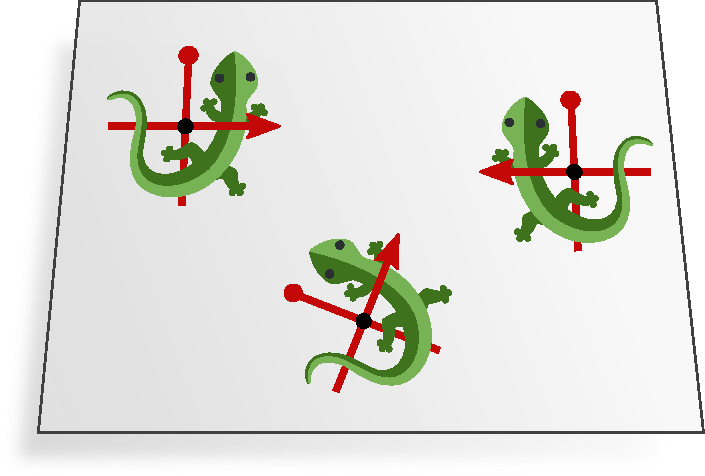
\includegraphics[width=.46\columnwidth]{figures/intro_lizard.pdf}
    \captionsetup{width=1\textwidth}
    \hspace{1.5ex}
    \caption{\small
        Typical patterns in signals appear commonly in different geometric poses.
        $\GM$-convolutions generalize over all poses that are related by the action of the chosen structure group~$G$.
        While a conventional CNN on ${M=\R^2}$ would have to learn to detect all lizards individually, a $\GM$-coordinate independent CNN would for $G=\SO2$ generalize between the left and bottom lizard and for $G=\Flip$ generalize between the left and right lizard.
        For $G=\O2$, it would be guaranteed to encode all three lizards as the \emph{same feature} in \emph{different poses}.
        {
        \color{gray}
        \scriptsize
            (Lizards adapted under the Creative Commons Attribution 4.0 International
            \href{https://github.com/twitter/twemoji/blob/gh-pages/LICENSE-GRAPHICS}{\underline{license}}
            by courtesy of Twitter.)
        }
        \\\protect\rule{0ex}{2.5ex}
        }
    \label{fig:intro_lizard}
\end{SCfigure}


A point that was so far left open is the choice of $G$-structure.
In general, a Riemannian manifold comes with a metric structure, i.e. an $\O{d}$-structure.
The reduction of the structure group to subgroups $G<\O{d}$ might be obstructed by the topology of the manifold
-- \emph{smooth} (or continuous) $G$-structures \emph{do not exist} if this is the case.
Except from this constraint, the choice of $G$-structure is mainly an engineering question, depending for instance on the desired equivariance properties.


In most applications
\marginnote{topological obstructions}
it is sensible to demand that the prediction of the neural network varies \emph{smoothly} over the manifold.
As $\GM$-convolutions share kernels relative to frames of some $G$-structure, the convolution response is only then guaranteed to be smooth when the $G$-structure is smooth.
It is a well known fact that the topology of a manifold obstructs the (smooth) reduction of its structure group beyond a certain level.
This implies that \emph{a minimum level of gauge equivariance is strictly necessary} for a smooth convolution operation.
We prove in Theorem~\ref{thm:existence_kernel_field_trafo_compact_kernels} that our $\GM$-convolutions are indeed preserving the smoothness of feature fields.


An intuitive example of such a topological obstruction is the non-orientability of the M\"obius strip from Fig.~\ref{fig:G_structure_intro_l}:
a reduction of the structure group to the trivial group $\{e\}$ would correspond to some choice of smooth frame field on the strip.
However, due to the twist of the strip, this reduction would necessarily lead to a discontinuity in form of a frame reflection at some point
-- a reduction to $G=\{e\}$ is therefore topologically obstructed and $\Flip$-steerable kernels are inevitable on the M\"obius strip.
Another example is the 2-sphere~$S^2$, which does not admit a reduction beyond~$G=\SO2$.


It is in the deep learning literature not uncommon
\marginnote{discontinuous networks}
to ignore such topological obstructions and to implement discontinuous networks.
An example are spherical CNNs which rely on the $\{e\}$-structure in Fig.~\ref{fig:G_structure_intro_k}; see Section~\ref{sec:spherical_CNNs_azimuthal_equivariant} for a detailed review of such models.
Note that a removal of the poles, where the frame field is singular, turns the spherical topology into a cylindrical topology, where a smooth reduction to $G=\{e\}$ is possible.
Section~\ref{sec:e_surface_conv} discusses further discontinuous $\GM$-convolutions which apply non-steerable kernels relative to heuristically (algorithmically) fixed $\{e\}$-structures.


It is important to understand that many different $G$-structures $\GM$ exist
\marginnote{non-uniqueness of $G$-structures}
for a given structure group~$G$ and manifold~$M$.
Figs.~\ref{fig:G_structure_intro_a} and~\ref{fig:G_structure_intro_b} show different choices of $\{e\}$-structures on $M=\R^2$ while
Figs.~\ref{fig:G_structure_intro_d} and~\ref{fig:G_structure_intro_e} show different $\Flip$-structures.
Different $\O{d}$-structures on $M$ correspond to different Riemannian metrics.
While the structure group~$G$ implies a kernel's $G$-steerability, the $G$-structure determines how exactly this kernel is to be shared.


Within the topological constraints,
\marginnote{global and local equivariance}
the structure group~$G$ and $G$-structure may be freely chosen by the user.
If the manifold comes with a non-trivial isometry group $\IsomM$, the $G$-structure $\GM$ is often designed such that the corresponding $\GM$-convolution is equivariant w.r.t. some subgroup~$\IsomGM$ of isometries.
Examples are given in Fig.~\ref{fig:G_structures_intro} and throughout our literature review in Part~\ref{part:literature_review}.
Even if the manifold is asymmetric, local patterns of features appear often in multiple different geometric poses.
The choice of structure group~$G$ provides a powerful tool to exploit such symmetries in the learning task:
$\GM$-convolutions generalize learned patterns automatically over any $G$-related pose; see Fig.~\ref{fig:intro_lizard}.
The optimal choice of structure group might thereby vary with the \emph{length scale} (field of view) and thus with the depth in the network~\cite{Weiler2019_E2CNN}.
For example, even though natural images are aligned on a global scale, local patterns like edges and corners usually appear in several directions, such that local gauge equivariance still proves to be useful.
